\documentclass[border=2pt]{standalone}
\usepackage{amsmath}
\usepackage{amsfonts}
\usepackage{amssymb}
\usepackage{tikz}
\usepackage{pgfplots}
\usepackage{circuitikz}
\usepackage{graphicx}
\usepackage{xcolor}
\usepackage[utf8]{inputenc}
\usepackage[T1]{fontenc}

% Bibliotecas TikZ
\usetikzlibrary{
  arrows,
  arrows.meta,
  positioning,
  shapes,
  shapes.geometric,
  shapes.multipart,
  calc,
  decorations.pathmorphing,
  decorations.markings,
  patterns,
  automata,
  trees,
  graphs,
  chains,
  fit,
  backgrounds,
  shadows
}

% Configurações PGFPlots
\pgfplotsset{compat=newest}

\begin{document}

    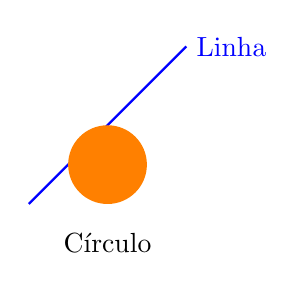
\begin{tikzpicture}
        % Desenha uma linha de (0,0) a (2,2)
        \draw[thick, blue] (0,0) -- (2,2) node[right] {Linha};
        
        % Desenha um círculo preenchido em laranja no ponto (1, 0.5) com raio de 0.5cm
        \fill[orange] (1, 0.5) circle (0.5cm);

        % Adiciona um nó de texto
        \node at (1, -0.5) {Círculo};
    \end{tikzpicture}
\end{document}
